\section{eo\-Reduce$<$ EOT $>$ Class Template Reference}
\label{classeo_reduce}\index{eoReduce@{eoReduce}}
eo\-Reduce: .reduce the new generation to the specified size At the moment, limited to truncation - with 2 different methods, one that sorts the whole population, and one that repeatidely kills the worst.  


{\tt \#include $<$eo\-Reduce.h$>$}

Inheritance diagram for eo\-Reduce$<$ EOT $>$::\begin{figure}[H]
\begin{center}
\leavevmode
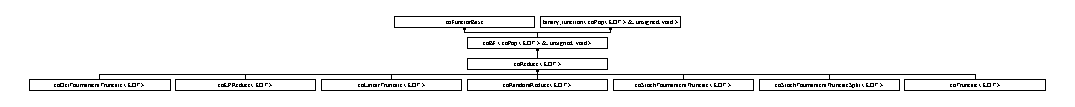
\includegraphics[height=0.987654cm]{classeo_reduce}
\end{center}
\end{figure}


\subsection{Detailed Description}
\subsubsection*{template$<$class EOT$>$ class eo\-Reduce$<$ EOT $>$}

eo\-Reduce: .reduce the new generation to the specified size At the moment, limited to truncation - with 2 different methods, one that sorts the whole population, and one that repeatidely kills the worst. 

Ideally, we should be able to choose at run-time!!! 



Definition at line 45 of file eo\-Reduce.h.

The documentation for this class was generated from the following file:\begin{CompactItemize}
\item 
eo\-Reduce.h\end{CompactItemize}
